% Vertical flow chart for the A0 portrait poster (poster_portrait.tex, 2026-09-23).
% Same content as system_pipeline.tex, stacked top to bottom and drawn at print size
% (units in mm, fonts in pt), so the poster includes it without scaling.
% Build from Poster/: latexmk -pdf -outdir=out system_pipeline_vertical.tex ;
% copy out/system_pipeline_vertical.pdf to figs/
\documentclass[tikz,border=1mm]{standalone}
\usepackage[T1]{fontenc}
\usepackage[utf8]{inputenc}
\usepackage{lato}
% lato.sty (2019) does not set a default family; select it by name, or text falls back to CM Sans.
\renewcommand{\sfdefault}{lato-TLF}
\renewcommand{\familydefault}{\sfdefault}
\usepackage{anyfontsize}
\usepackage{amsmath,amssymb}
\usetikzlibrary{arrows.meta,calc,positioning,decorations.pathreplacing}

\definecolor{dtured}{HTML}{990000}
\definecolor{dtugrey}{HTML}{666666}
\definecolor{dtulight}{HTML}{F1F1F1}
\definecolor{dtusand}{HTML}{F7F2EE}
\definecolor{dtupink}{HTML}{F7EAEA}
\definecolor{dtugold}{HTML}{F3E8CF}

\newcommand{\SHead}{\fontsize{44}{50}\selectfont\bfseries}
\newcommand{\SText}{\fontsize{30}{36}\selectfont}
\newcommand{\SMath}{\fontsize{42}{48}\selectfont}
\newcommand{\SSide}{\fontsize{28}{34}\selectfont}

% Vertical pitch between stage centres (mm); tune so the chart fills the column.
\newcommand{\pitch}{185}

\begin{document}
\hyphenpenalty=10000\exhyphenpenalty=10000
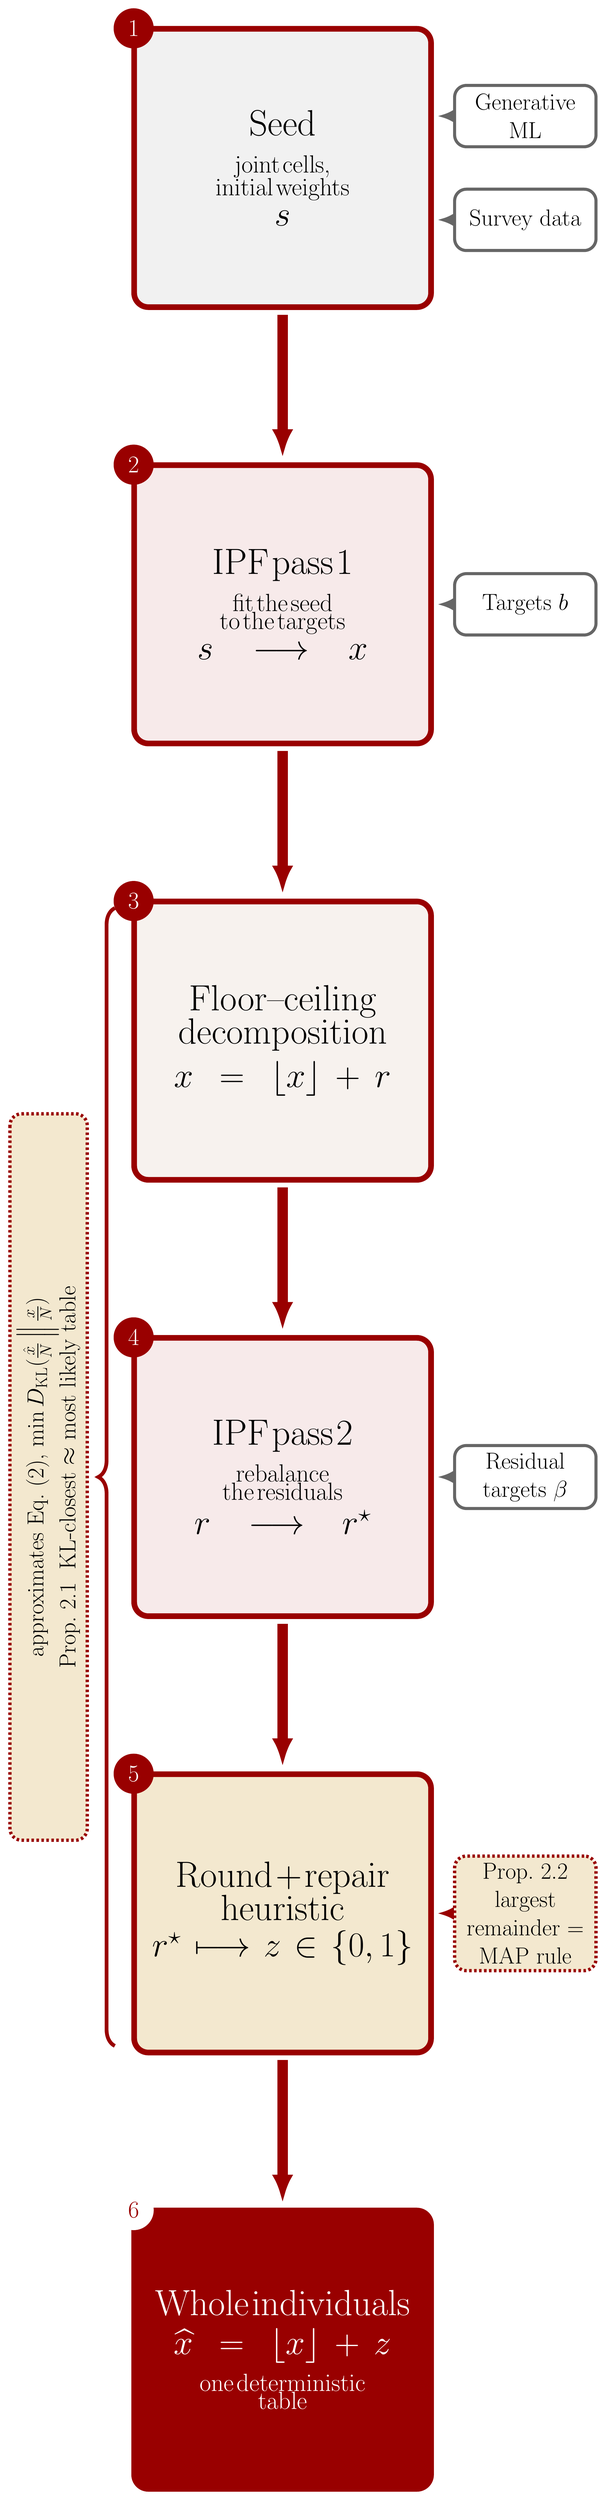
\begin{tikzpicture}[x=1mm, y=1mm,
  font=\sffamily,
  mainarrow/.style={-{Latex[length=12mm,width=9mm]}, draw=dtured,
                    line width=4.5mm, shorten <=2mm, shorten >=2mm},
  inputarrow/.style={-{Latex[length=7mm,width=5.5mm]}, draw=dtugrey,
                     line width=1.8mm, shorten >=1.5mm},
  proparrow/.style={-{Latex[length=7mm,width=5.5mm]}, draw=dtured,
                    line width=1.8mm, dashed, shorten >=1.5mm},
  stage/.style={draw=dtured, line width=2.4mm, rounded corners=6mm,
                minimum width=126mm, minimum height=118mm,
                text width=116mm, align=center, inner sep=4mm},
  input/.style={draw=dtugrey, line width=1.3mm, rounded corners=5mm,
                fill=white, minimum height=26mm, text width=52mm, align=center,
                font=\SSide\bfseries, inner xsep=4mm, inner ysep=3mm},
  prop/.style={draw=dtured, line width=1.4mm, dashed, rounded corners=5mm,
               fill=dtugold, align=center, font=\SSide,
               inner xsep=4mm, inner ysep=3mm},
  stepbadge/.style={circle, fill=dtured, text=white, minimum size=17mm,
                    inner sep=0pt, font=\fontsize{29}{35}\selectfont\bfseries},
  outbadge/.style={circle, fill=white, text=dtured, minimum size=17mm,
                   inner sep=0pt, font=\fontsize{29}{35}\selectfont\bfseries}
]

% Main stages, stacked top to bottom (x centre 113 mm).
\node[stage, fill=dtulight] (seed) at (113,0) {%
  {\SHead Seed}\par\vspace{3mm}
  {\SText joint cells,\\ initial weights}\par\vspace{4mm}
  {\SMath $s$}};
\node[stage, fill=dtupink] (ipfone) at (113,-\pitch) {%
  {\SHead IPF pass 1}\par\vspace{3mm}
  {\SText fit the seed\\ to the targets}\par\vspace{4mm}
  {\SMath $s \longrightarrow x$}};
\node[stage, fill=dtusand] (split) at (113,-2*\pitch) {%
  {\SHead Floor--ceiling\par decomposition}\par\vspace{4mm}
  {\SMath $x=\lfloor x\rfloor+r$}};
\node[stage, fill=dtupink] (ipftwo) at (113,-3*\pitch) {%
  {\SHead IPF pass 2}\par\vspace{3mm}
  {\SText rebalance\\ the residuals}\par\vspace{4mm}
  {\SMath $r \longrightarrow r^{\star}$}};
\node[stage, fill=dtugold] (round) at (113,-4*\pitch) {%
  {\SHead Round + repair\par heuristic}\par\vspace{4mm}
  {\SMath $r^{\star}\longmapsto z\in\{0,1\}$}};
\node[stage, fill=dtured, text=white] (people) at (113,-5*\pitch) {%
  {\SHead Whole individuals}\par\vspace{5mm}
  {\SMath $\widehat{x}=\lfloor x\rfloor+z$}\par\vspace{3mm}
  {\SText one deterministic\\ table}};

% Stage numbers.
\foreach \n/\lab in {seed/1, ipfone/2, split/3, ipftwo/4, round/5}
  \node[stepbadge] at ($(\n.north west)+(1,-1)$) {\lab};
\node[outbadge] at ($(people.north west)+(1,-1)$) {6};

% Main flow.
\draw[mainarrow] (seed.south) -- (ipfone.north);
\draw[mainarrow] (ipfone.south) -- (split.north);
\draw[mainarrow] (split.south) -- (ipftwo.north);
\draw[mainarrow] (ipftwo.south) -- (round.north);
\draw[mainarrow] (round.south) -- (people.north);

% External inputs, to the right of the stage they feed.
\node[input] (ml) at (216,22) {Generative ML};
\node[input] (survey) at (216,-22) {Survey data};
\draw[inputarrow] (ml.west) -- ($(seed.east)+(0,22)$);
\draw[inputarrow] (survey.west) -- ($(seed.east)+(0,-22)$);
\node[input] (targets) at (216,-\pitch) {Targets $b$};
\draw[inputarrow] (targets.west) -- (ipfone.east);
\node[input] (rtargets) at (216,-3*\pitch) {Residual\\targets $\beta$};
\draw[inputarrow] (rtargets.west) -- (ipftwo.east);

% Propositions. Prop. 2.2 concerns the rounding step (box 5); Prop. 2.1 concerns
% the objective Eq. (2), which steps 3-5 together approximate (bracket, left).
\node[prop, text width=52mm] (p22) at (216,-4*\pitch)
  {\textbf{Prop.\ 2.2}\\ largest remainder $=$ MAP rule};
\draw[proparrow] (p22.west) -- (round.east);
\draw[decorate, decoration={brace, amplitude=7mm}, draw=dtured,
      line width=1.6mm]
  ($(round.south west)+(-7,4)$) -- ($(split.north west)+(-7,-4)$)
  coordinate[midway] (bmid);
\node[prop, rotate=90, anchor=south, text width=300mm] at ($(bmid)+(-11,0)$)
  {approximates Eq.\ (2), $\min D_{\mathrm{KL}}(\frac{\hat{x}}{N}\,\Big\|\,\frac{x}{N})$\\
   \textbf{Prop.\ 2.1}\; KL-closest $\approx$ most likely table};
\end{tikzpicture}
\end{document}